\documentclass[11pt]{amsart}
\usepackage[a4paper,margin=1in]{geometry}
\usepackage{amsmath,amssymb,amsthm}
\usepackage{booktabs}
\usepackage{tikz}
\usepackage[hidelinks]{hyperref}

\newtheorem{theorem}{Theorem}[section]
\newtheorem{lemma}[theorem]{Lemma}
\newtheorem{proposition}[theorem]{Proposition}
\newtheorem{corollary}[theorem]{Corollary}
\theoremstyle{definition}
\newtheorem{definition}[theorem]{Definition}
\newtheorem{remark}[theorem]{Remark}

\newcommand{\C}{\mathbb{C}}
\newcommand{\PP}{\mathbb{P}}
\newcommand{\Div}{\operatorname{div}}
\newcommand{\ord}{\operatorname{ord}}
\newcommand{\Res}{\operatorname{Res}}

\title[Genus-one curves on the magic-square-of-squares surface]{Genus-one curves of low degree on the surface of
three-by-three magic squares of squares}
\author{Vamshi Jandhyala}
\address{London, United Kingdom}
\email{vamshi.jandhyala@gmail.com}
\subjclass[2020]{14J29, 14H52, 11D25}
\keywords{magic square of squares, surface of general type, elliptic curve, Bombieri--Lang conjecture}
\date{Preprint v1, 22 November 2026}

\begin{document}

\begin{abstract}
Auel and Singer showed that $3\times3$ magic squares of squares are rational points on a surface $V\subset\PP^8$ of
general type, cut out by six quadrics, and that the hyperplane section where the centre entry vanishes contains
sixteen elliptic curves of degree four. By the Bombieri--Lang conjecture, all but finitely many rational points of
$V$ lie on curves of genus zero or one, so these curves are where magic squares of squares could be found in
abundance. We prove that the sixteen curves are the only curves of geometric genus one on $V$ of degree at most six.
The proof attaches to such a curve four rational functions, one for each line through the centre of the square, and
derives a list of necessary conditions on their divisors: a genus-five obstruction, forced ramification at the zeros
of the centre coordinate, the group law of the elliptic curve, and a square-class obstruction for pencils of degree
two. In degrees five and six the conditions leave no configuration. Every exclusion was recomputed by independently
written code, and the group-law exclusions and the last stage carry certificates checked by separate code. In degree seven the same method reduces $8280$ configurations to $110$, all of one
type.
\end{abstract}

\maketitle

\section{Introduction}

Nobody knows whether there is a $3\times3$ magic square whose nine entries are distinct perfect squares. The question is
about a surface: Michaud-Rodgers \cite{MR} studied it as a projective variety in an undergraduate dissertation,
finding its $256$ singular points and showing that it contains no lines, and Auel and Singer \cite{AS} developed
its geometry in detail. The nine entries of a $3\times3$ magic square with centre $e$ are
the numbers $e+au+bv$ for $(a,b)\in\{-1,0,1\}^2$, for suitable $u$ and $v$, so a magic square of squares is a point of the surface
\[
V=\{\,[t_{ab}]\in\PP^8 : t_{ab}^2=e+au+bv \text{ for some } e,u,v \text{ and all } (a,b)\in\{-1,0,1\}^2\,\}
\]
with rational coordinates. Eliminating $e=t_{00}^2$, $u=t_{10}^2-t_{00}^2$ and $v=t_{01}^2-t_{00}^2$ leaves six
quadrics, and $V$ is their intersection. It has $256$ ordinary double points, its resolution is of general type
\cite{AS}, and the Bombieri--Lang conjecture then predicts that its rational points lie on finitely many curves
of genus zero or one, apart from finitely many others. Classifying those curves is the geometric half of the problem.

The curves we know come from the centre. On the hyperplane $t_{00}=0$ we have $e=0$, so $t_{ab}^2=au+bv$. Write
$x=t_{10}$, $y=t_{01}$, $z=t_{11}$ and $w=t_{1,-1}$. Then $u=x^2$ and $v=y^2$, each of the four remaining
coordinates is $\pm i$ times one of $x,y,z,w$ (for instance $t_{-1,0}^2=-u$), and the curve
\[
z^2=x^2+y^2,\qquad w^2=x^2-y^2
\]
in $\PP^3$ is a smooth elliptic curve of degree four. Auel and Singer show that the section $t_{00}=0$ is the union
of sixteen such curves, one for each choice of the signs \cite{AS}. Bruin, Thomas and
V\'arilly-Alvarado \cite{BTVA} proved that $V$ is algebraically quasi-hyperbolic: it contains only finitely many curves
of genus zero or one. Their method does not list the curves. In an unrefereed document \cite{Dz}, Dzoba showed that
every rational curve on $V$ is one of the $128$ conics found by Auel and Singer; our independent check of that
argument is included in the data of this paper. For curves of degree at most two the same conclusion was reached
independently by the MagicNumbers project \cite{MN}: $V$ contains no lines and exactly $128$ conics. The same document
\cite{Dz} studies genus one through the plane image $C$ of the curve under $[e:u:v]$: apart
from the sixteen quartics, $C$ has degree at least four, and at least six if its normalisation is elliptic; part of
the case of rational plane quartics is excluded; and an application of Miyaoka's inequality to the orbit of the curve
on a double cover of $V$ bounds the degree of $C$ by $153$, which makes the classification a finite problem without
settling it. For the analogous surface parametrising perfect cuboids, Stoll and Testa \cite{ST} classified all
integral curves of degree at most six, by a different method: the Picard group of the resolution and a K3 quotient.

\begin{theorem}\label{thm:main}
Let $D\subset V$ be an irreducible curve whose normalisation has genus one. If $\deg D\le 6$, then $D$ is one of the
sixteen quartics in the hyperplane $t_{00}=0$.
\end{theorem}

Degree here is the hyperplane degree of $D$, which equals the degree of the pull-back of $\mathcal O(1)$ to the
normalisation. In degree seven the same method leaves $110$ of $8280$ configurations, all with the same shape
(Section~\ref{sec:seven}).

\subsection*{The route}
A genus-one curve with $t_{00}\not\equiv0$ meets the centre hyperplane in a divisor $\theta$ of degree $m=\deg D$.
For each of the four lines through the centre of the square, the two opposite entries $A$, $B$ satisfy
$A^2+B^2=2t_{00}^2$, which factors over $\C$ as $(A+iB)(A-iB)=2t_{00}^2$. So the quotient $(A+iB)/(\sqrt2\,t_{00})$ is
a rational function on the elliptic curve whose zeros and poles lie in $\theta$. This gives four functions
$\phi_1,\dots,\phi_4$ and four integer vectors, their divisors. The surface equations become two identities
\eqref{eq:rel} between the functions $\phi_i^2+\phi_i^{-2}$. Everything after that extracts necessary conditions from
these identities: which divisors are possible locally (Lemma~\ref{lem:full}), which are possible globally
(Sections~\ref{sec:distinct} to \ref{sec:pencil}), and whether the points can be placed on an elliptic curve at all
(the group law). In low degree the conditions leave nothing. Figure~\ref{fig:grid} shows the four pairs and a degree-four
divisor table.

\section{Centre-pair functions}\label{sec:setup}

\begin{figure}[t]
\centering
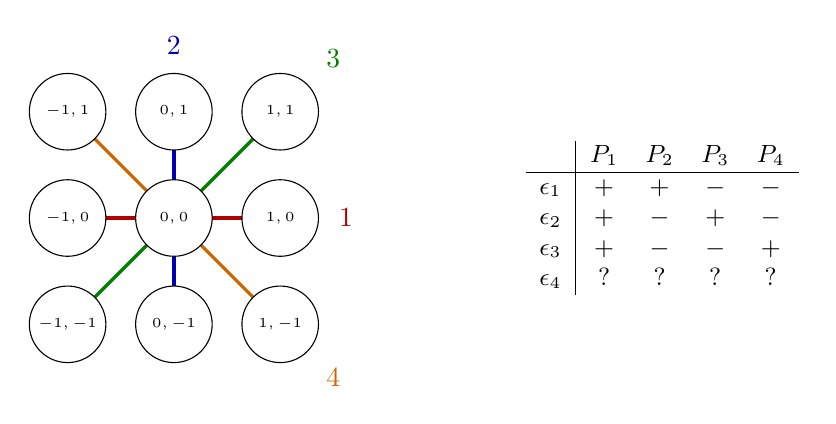
\begin{tikzpicture}
  \begin{scope}[scale=1.35]
  \draw[very thick,red!70!black] (-1.36,0)--(1.36,0);
  \draw[very thick,blue!70!black] (0,-1.36)--(0,1.36);
  \draw[very thick,green!50!black] (-1.25,-1.25)--(1.25,1.25);
  \draw[very thick,orange!80!black] (-1.25,1.25)--(1.25,-1.25);
  \foreach \a in {-1,0,1} \foreach \b in {-1,0,1}
    {\filldraw[fill=white,draw=black] (\a,\b) circle (0.36); \node at (\a,\b) {\tiny $\a,\b$};}
  \node[red!70!black] at (1.62,0) {$1$}; \node[blue!70!black] at (0,1.62) {$2$};
  \node[green!50!black] at (1.5,1.5) {$3$}; \node[orange!80!black] at (1.5,-1.5) {$4$};
  \end{scope}
  \begin{scope}[xshift=6.2cm]
    \node at (0,0) {\small
      $\begin{array}{c|cccc}
        & P_1 & P_2 & P_3 & P_4\\ \hline
        \epsilon_1 & + & + & - & -\\
        \epsilon_2 & + & - & + & -\\
        \epsilon_3 & + & - & - & +\\
        \epsilon_4 & ? & ? & ? & ?
      \end{array}$};
  \end{scope}
\end{tikzpicture}
\caption{Left: the nine cells $(a,b)$ of the square and the four pairs of opposite cells through the centre. Right:
why degree four forces the known quartics. Each row is the divisor of a centre-pair function on $\theta=P_1+\dots+P_4$
and splits $\theta$ into two halves of degree two. There are only three such splittings, so the fourth row repeats one
of the others up to sign, which the genus-five obstruction forbids (Proposition~\ref{prop:distinct},
Corollary~\ref{cor:low}).}
\label{fig:grid}
\end{figure}

Number the pairs through the centre as in Figure~\ref{fig:grid} and choose one cell $A_i$ of each pair, with $B_i$
the opposite cell:
\begin{align*}
(A_1,B_1)&=(t_{10},t_{-1,0}), & (A_2,B_2)&=(t_{01},t_{0,-1}),\\
(A_3,B_3)&=(t_{11},t_{-1,-1}), & (A_4,B_4)&=(t_{1,-1},t_{-1,1}).
\end{align*}
Put $M=t_{00}$. The surface equations give $A_i^2+B_i^2=2e=2M^2$ and
\[
A_1^2-B_1^2=2u,\quad A_2^2-B_2^2=2v,\quad A_3^2-B_3^2=2(u+v),\quad A_4^2-B_4^2=2(u-v).
\]

Let $D\subset V$ be an irreducible curve with normalisation $\nu\colon E\to D$ of genus one, and put
$N=\nu^*\mathcal O(1)$, of degree $m=\deg D$. The pulled-back coordinates are sections of $N$ with no common zero.
Suppose $M\not\equiv0$ on $D$, and write $\theta=\Div(M)=\sum_P\mu_PP$, an effective divisor of degree $m$. Define
\[
\phi_i=\frac{A_i+iB_i}{\sqrt2\,M},\qquad h_i=\phi_i^2+\phi_i^{-2}=\frac{A_i^2-B_i^2}{M^2}.
\]
The second expression for $h_i$ uses $\phi_i^{-1}=(A_i-iB_i)/(\sqrt2M)$, which holds because
$(A_i+iB_i)(A_i-iB_i)=2M^2$. Reading the four offsets off the equations above gives
\begin{equation}\label{eq:rel}
h_3=h_1+h_2,\qquad h_4=h_1-h_2.
\end{equation}
These two identities are all we use about $V$ until Section~\ref{sec:seven}.

Since $\ord_P(A_i+iB_i)+\ord_P(A_i-iB_i)=2\mu_P$ with both terms nonnegative, the integer
$\epsilon_{iP}=\ord_P\phi_i$ satisfies $|\epsilon_{iP}|\le\mu_P$, and $\phi_i$ has no zeros or poles outside
$\theta$. Call the pair $i$ \emph{full} at $P$ if $|\epsilon_{iP}|=\mu_P$. The degree of $\phi_i$ is
$k_i=\sum_P\max(\epsilon_{iP},0)=\tfrac12\sum_P|\epsilon_{iP}|\le m/2$, and $k_i\ne1$ because an elliptic curve has
no function of degree one.

\begin{lemma}\label{lem:full}
At every point $P$ of $\theta$, at least three of the four pairs are full.
\end{lemma}

\begin{proof}
Some coordinate $t_{ab}$ is nonzero at $P$; it is not $M$, so it lies in a pair $i$, and then one of $A_i\pm iB_i$
is nonzero at $P$, so the pair is full. Hence the largest $|\epsilon_{iP}|$ equals $\mu_P$. The function $h_i$ has a
pole of order exactly $2|\epsilon_{iP}|$ at $P$ if $\epsilon_{iP}\ne0$ and no pole otherwise. Any three of
$h_1,\dots,h_4$ satisfy a linear relation with nonzero coefficients, by \eqref{eq:rel}, so in every three the
largest pole order is attained at least twice. If two pairs were not full, the three formed by them and one full pair
would attain the largest pole order only once.
\end{proof}

\begin{definition}
The \emph{table} of $D$ is the list of columns $(\mu_P;\epsilon_{1P},\dots,\epsilon_{4P})$, one for each point of
$\theta$, up to reordering the points and changing the sign of a row (replacing $\phi_i$ by $\phi_i^{-1}$, which leaves
$h_i$ unchanged).
\end{definition}

A table satisfies: the $\mu_P$ add up to $m$; each column has $|\epsilon_{iP}|\le\mu_P$ with at least three equalities;
each row sums to zero and has $k_i\ne1$. We call such a table \emph{admissible}. For each $m$ there are finitely many,
and the proof of Theorem~\ref{thm:main} shows that none of them comes from a curve when $5\le m\le 6$.

The group law gives the first global condition. A divisor of degree zero on an elliptic curve is principal exactly
when its points add up to zero in the group law \cite[Cor.~III.3.5]{Si}. Each row of a table is principal, and so is
every integer combination of rows. Fix one point of $\theta$ as the origin. Whether some choice of distinct points on
some elliptic curve satisfies a given list of such relations is a question about the integer relation matrix: its
Smith normal form splits the solutions into a torsion part and a free part, and the points are forced to coincide
exactly when, for every torsion choice, two points have the same free part and the same torsion part. We call a table
that fails this test \emph{excluded by the group law}.

\section{Two obstructions valid in every degree}\label{sec:distinct}

\begin{proposition}\label{prop:nonconst}
If $M\not\equiv0$ on $D$, no $\phi_i$ is constant.
\end{proposition}

\begin{proof}
If $\phi_i$ is constant then so is $h_i$, so one of $u/e$, $v/e$, $(u+v)/e$, $(u-v)/e$ is constant on $D$. The map
$V\to\PP^2$, $[t]\mapsto[e:u:v]$, is the quotient by the sign changes of the nine coordinates, so it is finite, and
$D$ is a component of the preimage of a line $L$ of the form $u=ce$, $v=ce$, $u+v=ce$ or $u-v=ce$. The symmetries of
the square exchange $u$ and $v$ and change the sign of $v$, so two kinds of line suffice: $u=ce$ and $u+v=ce$.
Parametrise $L$ by $z=v/e$ or $z=u/e$. Each ratio $t_{ab}^2/t_{00}^2$ restricts to a constant or to a polynomial of
degree one in $z$. If the nonconstant ones have $n$ distinct roots, each component of the preimage is the
$(\mathbb Z/2)^n$ cover of $L$ obtained by adjoining the square roots of $z-\alpha$ for the roots $\alpha$; it is
branched with index two over the $n$ roots and over $z=\infty$, and nowhere else. Riemann--Hurwitz gives genus
$1+2^{n-2}(n-3)$. For $u=ce$ the roots are $\pm1$, $\pm(1+c)$, $\pm(1-c)$, so $n=2$ for $c=0$, $n=5$ for $c=\pm1$,
$n=4$ for $c=\pm2$, and $n=6$ otherwise. For $u+v=ce$ the roots are $1$, $-1$, $c\pm1$, $(c\pm1)/2$, so $n=4$ for
$c\in\{0,\pm1,\pm3\}$, $n=5$ for $c=\pm2$, and $n=6$ otherwise. In no case is $n=3$, so no component has genus one.
\end{proof}

\begin{lemma}[genus five]\label{lem:g5}
Let $K$ be the function field of an elliptic curve, let $f,g\in K^\times$ with $f$ nonconstant, and suppose
$g^2+g^{-2}=af^2+bf^{-2}$ with $a,b\in\C$. Then $ab\in\{0,1\}$.
\end{lemma}

\begin{proof}
Suppose $a,b\ne0$ and $ab\ne1$, and put $H=ax^2+bx^{-2}\in\C(x)$. The numerators of $H+2$ and $H-2$ are
$ax^4+2x^2+b$ and $ax^4-2x^2+b$. Each has discriminant $256\,ab(ab-1)^2\ne0$, their zeros are disjoint and nonzero,
and the poles of $H\pm2$ at $0$ and $\infty$ have even order. So $F=\C(x)(\sqrt{H+2},\sqrt{H-2})$ is a biquadratic
extension branched at eight points with index two, and Riemann--Hurwitz gives $2g(F)-2=4(-2)+8\cdot2=8$, that is,
$g(F)=5$. Since $(g\pm g^{-1})^2=H(f)\pm2$, the assignments $x\mapsto f$, $\sqrt{H+2}\mapsto g+g^{-1}$,
$\sqrt{H-2}\mapsto g-g^{-1}$ define a homomorphism of fields $F\to K$, which is injective. A curve of genus one
does not dominate a curve of genus five, so this is impossible.
\end{proof}

When $ab=1$, choosing $\alpha^2=a$ gives $Y^4-(af^2+bf^{-2})Y^2+1=(Y^2-af^2)(Y^2-bf^{-2})$, so $g\in\C(f)$; the lemma
allows this case and the case where one coefficient vanishes, and the next proof handles both.

\begin{proposition}\label{prop:distinct}
If $M\not\equiv0$ on $D$, the four divisors $\Div\phi_i$ are pairwise distinct, even up to sign.
\end{proposition}

\begin{proof}
Suppose $\Div\phi_j=\pm\Div\phi_i$. Inverting $\phi_j$ if necessary, $\phi_j=c\,\phi_i$ for a constant $c$. Put
$f=\phi_i$, $t=c^2$ and $z=t+t^{-1}$. Then $h_i=f^2+f^{-2}$ and $h_j=tf^2+t^{-1}f^{-2}$, and by \eqref{eq:rel} each of
the two remaining $h_\ell$ equals $A_\ell f^2+B_\ell f^{-2}$. By Lemma~\ref{lem:g5} both products $A_\ell B_\ell$ lie
in $\{0,1\}$. Substituting gives the products in the following table.
\begin{center}\small
\begin{tabular}{lll}
\toprule
repeated pair $\{i,j\}$ & products $A_\ell B_\ell$ & values of $z$ allowed\\
\midrule
$\{1,2\}$ & $2+z$, $2-z$ & none\\
$\{3,4\}$ & $(2+z)/4$, $(2-z)/4$ & $\pm2$\\
$\{1,3\}$, $\{1,4\}$, $\{2,3\}$ & $2-z$, $5-2z$ & $2$\\
$\{2,4\}$ & $2+z$, $5+2z$ & $-2$\\
\bottomrule
\end{tabular}
\end{center}
For instance, for $\{1,3\}$ the relations give $h_2=h_3-h_1$ and $h_4=2h_1-h_3$, with products
$(t-1)(t^{-1}-1)=2-z$ and $(2-t)(2-t^{-1})=5-2z$. When $z=\pm2$ we have $t=\pm1$, and in every allowed case one of
the remaining $h_\ell$ vanishes identically, so $\phi_\ell^4=-1$ and $\phi_\ell$ is constant, contrary to
Proposition~\ref{prop:nonconst}.
\end{proof}

\begin{corollary}\label{cor:low}
Theorem~\ref{thm:main} holds for $\deg D\le4$.
\end{corollary}

\begin{proof}
If $M\equiv0$ on $D$, then $D$ lies in the section $t_{00}=0$, which is the union of the sixteen quartics
\cite{AS}, so $D$ is one of them. Suppose $M\not\equiv0$. Each $k_i$ is at most $m/2$, nonzero by
Proposition~\ref{prop:nonconst}, and not one. For $m\le3$ this is impossible. For $m=4$ every $k_i=2$, so
$\sum_P|\epsilon_{iP}|=4=\sum_P\mu_P$ and every pair is full at every point. Each row then splits $\theta$ into two
halves of degree two, with sign $+$ on one half and $-$ on the other. A divisor of degree four has at most three such
splittings up to exchanging the halves (three when its points are distinct, one when it is $2P+Q+R$ or $2P+2Q$, none
otherwise). Four rows and at most three splittings force two rows to agree up to sign
(Figure~\ref{fig:grid}), contradicting Proposition~\ref{prop:distinct}.
\end{proof}

\section{Forced ramification}\label{sec:ram}

At a point where one pair is not full, the identities \eqref{eq:rel} fix the leading coefficients of the other three
functions up to a common factor, and this forces certain monomials in the $\phi_i$ to take known values with
multiplicity.

Write $H_1=(1,0)$, $H_2=(0,1)$, $H_3=(1,1)$, $H_4=(1,-1)$, so that $h_\ell$ is the dot product of $H_\ell$ with
$(h_1,h_2)$.

\begin{lemma}\label{lem:forced}
Let $P\in\theta$, and let $i,j,c$ be distinct with $|\epsilon_{iP}|=|\epsilon_{jP}|=\mu>|\epsilon_{cP}|$. Write
$s_i,s_j\in\{\pm1\}$ for the signs of $\epsilon_{iP},\epsilon_{jP}$, let $w$ be a nonzero vector perpendicular to
$H_c$, and put $r=(H_j\cdot w)/(H_i\cdot w)$. Then the monomial $f=\phi_i^{s_i}\phi_j^{-s_j}$ is a unit at $P$,
$f(P)^2=r$, and $\ord_P(f-f(P))\ge2(\mu-|\epsilon_{cP}|)$.
\end{lemma}

\begin{proof}
In a local coordinate $z$ at $P$, $h_i$ and $h_j$ have poles of order exactly $2\mu$ with leading terms
$\phi_i^{-2s_i}$ and $\phi_j^{-2s_j}$, the other term in each being smaller by a factor of order $4\mu$. The third
function $h_c$ has a pole of order at most $2|\epsilon_{cP}|<2\mu$. The linear relation among $h_i,h_j,h_c$ from
\eqref{eq:rel} gives $h_j/h_i=r+O(z^{2(\mu-|\epsilon_{cP}|)})$, while $h_j/h_i=f^2(1+O(z^{4\mu}))$. Since $r\ne0$,
$f+f(P)$ is a unit and the bound passes from $f^2$ to $f$.
\end{proof}

We call $P$ a \emph{forced point} of $f$, with value $f(P)^2$ and multiplicity
$r_P=2(\mu-|\epsilon_{cP}|)$. Let $f$ be such a monomial, of degree $\delta>0$ with divisor $d=\sum d_PP$. The
following hold.
\begin{enumerate}
\item[(R1)] (Riemann--Hurwitz) $\sum_{d_P\ne0}(|d_P|-1)+\sum_{\text{forced }P}(r_P-1)\le2\delta$.
\item[(R2)] (one fibre) $r_P\le\delta$ for every forced point.
\item[(R3)] (two fibres) the forced points with a common value $z$ lie in the two fibres $f=\pm\sqrt z$, so their
multiplicities add up to at most $2\delta$.
\item[(R4)] (full fibre) if $r_P=\delta$, the fibre through $P$ is $\delta P$, so $Z_f-\delta P$ is principal, where
$Z_f$ is the zero divisor of $f$.
\end{enumerate}
If $\delta=0$, then $f$ is constant and all its forced values must agree. Condition (R4) adds rows to the relation
matrix of the group law. The conditions apply to all six pairs $\{i,j\}$, and to both monomials
$\phi_i\phi_j^{\pm1}$ of each pair.

\section{A square-class obstruction for pencils of degree two}\label{sec:pencil}

The last three conditions use the Riemann--Roch space of a point of multiplicity two.

\begin{lemma}\label{lem:pencil}
Suppose that, after inverting some of them, three centre-pair functions are $\psi_A=fw$, $\psi_B=gw$ and $\psi_C=w$,
where $w$ has odd degree and $\Div f=2P-2R$, $\Div g=2Q-2R$ for distinct points $P,Q,R$. Let
$a\,h_A+b\,h_B+c\,h_C=0$ be the relation from \eqref{eq:rel}, and suppose the values $F=f(Q)^2$ and $G=g(P)^2$ are
known and nonzero. Then
\[
R(X)=-\,\frac{a/(FX^2)+b/(G(X-1)^2)+c}{aFX^2+bG(X-1)^2+c}
\]
is a square in $\C(X)$, provided its denominator is not identically zero.
\end{lemma}

\begin{proof}
The space of functions with at most a double pole at $R$ has dimension two, with basis $1,f$, so $g$ is affine in
$f$. As $f(P)=0$ and $g(Q)=0$, with $\alpha=f(Q)$ and $\beta=g(P)$, we get $g=\beta(1-X)$ for $X=f/\alpha$, a function
of degree two. Multiplying the relation by $w^2$ gives $w^4=R(X)$. The field $K$ of $E$ has degree two over
$B=\C(X)$, and $w\notin B$ because every element of $B$ has even degree on $E$. Let $\sigma$ generate
$\operatorname{Gal}(K/B)$. Since $w^4\in B$, $\sigma(w)=\zeta w$ with $\zeta^4=1$; applying $\sigma$ twice gives
$\zeta^2=1$, and $\zeta=1$ would put $w$ in $B$. So $\sigma(w)=-w$, $w^2\in B$, and $R=(w^2)^2$.
\end{proof}

The values $F$ and $G$ come from Lemma~\ref{lem:forced}. When only $G$ is forced, a further forced point $T$ of both
$f$ and $g$ with $g(T)^2=G$ recovers $F$: the fibre of $g$ over $\beta$ is $2P$, so $g(T)=-\beta$, hence $X(T)=2$ and
$F=f(T)^2/4$. The symmetric rule recovers $G$ from $F$. A rational function is a square in $\C(X)$ only if every
irreducible factor of its reduced numerator and denominator has even multiplicity, which an exact factorisation over
$\mathbb Q$ decides.

Two more arguments are needed in degree six, each for one table.

\begin{lemma}[three affine functions]\label{lem:affine}
No table has degrees $(3,3,3,3)$ with, after inverting some rows, $\Div(\psi_\ell/\psi_1)=2P_\ell-2R$ for
$\ell=2,3,4$, the points $P_2,P_3,P_4,R$ distinct.
\end{lemma}

\begin{proof}
Put $w=\psi_1$ and $f,g,h=\psi_2/w,\psi_3/w,\psi_4/w$. These lie in the two-dimensional space of functions with at
most a double pole at $R$, so they are affine functions of one function $x$ of degree two, with distinct simple zeros
in $x$. Multiplying \eqref{eq:rel} by $w^2$ gives
\[
w^4=\frac{1+f^{-2}-g^{-2}}{g^2-1-f^2}=\frac{1-f^{-2}-h^{-2}}{h^2-1+f^2}.
\]
Neither denominator vanishes identically, since $(g-f)(g+f)=1$ or $(h+if)(h-if)=1$ would make $f$ constant. At the
zero of $g$ the first quotient has a pole of order at least two in $x$, while the numerator of the second is regular
there, so its denominator, a polynomial of degree at most two in $x$, is $\kappa g^2$. Symmetrically
$g^2-1-f^2=\lambda h^2$. Adding gives $(1-\kappa)g^2+(1-\lambda)h^2=2$. Comparing the coefficients of $x^2$ and $x$
in this identity, with $g$ and $h$ affine with different zeros, forces both coefficients to vanish, and then $0=2$.
\end{proof}

\begin{lemma}[a monomial relation]\label{lem:mono}
Suppose that, after inverting some rows, $\psi_1\psi_4=c\,\psi_2\psi_3$ for a constant $c$ and that
$\psi_1/\psi_2$ has degree two. Then the identities \eqref{eq:rel} have no solution.
\end{lemma}

\begin{proof}
Put $w=\psi_1$, $f=\psi_1/\psi_2$, $g=\psi_1/\psi_3$, $t=\psi_1\psi_4$, $a=c^2$, and $F=f^2$, $G=g^2$,
$T=t^2$. Then $w^2=tfg/c$, and multiplying \eqref{eq:rel} through gives
\begin{equation}\label{eq:mono}
T(FG+G-F)+a(1+F-G)=0,\qquad T(FG-G-a)+a(1-F)-FG=0.
\end{equation}
Eliminating $T$ gives $\mathcal A G^2+\mathcal B G+\mathcal C=0$ with
$\mathcal A=-F^2+(a-1)F-a$, $\mathcal B=(1-2a)F^2-a^2+2a$, $\mathcal C=aF^2+(a^2-a)F+a^2$, and discriminant
$\Delta=(4a^2+1)F^4+6a^2F^2+a^4+4a^2$. Let $B_0=\C(f)$, so $[K:B_0]=2$. As a quadratic in $f^4$, $\Delta$ has
discriminant $-16b(b+1)^2$ with $b=a^2$; checking the special values $b=-\tfrac14,-4,-1$ shows that $\Delta$ is a
square in $B_0$ exactly when $a=\pm i$, where $\Delta=-3(F^2+1)^2$. (The eliminations, discriminants, resultants and
factorisations in this proof are omitted here; the program \texttt{verify\_sec5.py} in the data deposit recomputes
them exactly.)

If $\Delta$ is not a square, $B_0(G)=K$, and with $q$ the norm and $p$ the trace of $g$ from $K$ to $B_0$ we get
$q^2=\mathcal C/\mathcal A$ and $p^2=-\mathcal B/\mathcal A+2q$. Since $\operatorname{Res}_F(\mathcal A,\mathcal C)
=4a^3(a-1)^2$ and the constant terms are nonzero, $\mathcal A\mathcal C$ is a square only if $a=1$ or both quadratics
have double roots, which happens for $a^2-6a+1=0$. For $a=1$, $q=\pm i$ and
$p^2=((2q-1)f^4+2q+1)/(f^4+1)$ has four simple poles. For $a=3\pm2\sqrt2$, with $r=(a-1)/2$, one finds
$\mathcal A=-(F-r)^2$, $\mathcal C=a(F+r)^2$, and $p^2=(Lf^4+M')/(f^2-r)^2$ with $L,M'$ nonzero (their imaginary
parts are nonzero), whose numerator has four simple roots. In each case $p^2$ is not a square in $B_0$.

If $a=i$, the quadratic formula and the first identity in
\eqref{eq:mono} give, with $r=(\sqrt3-1)/2$ and $s=(\sqrt3+1)/2$ and nonzero constants $k,\ell$,
\[
G=k\,\frac{F+r(1-i)}{F+s(1-i)},\qquad T=\ell\,\frac{F+s(1+i)}{F+r(1+i)}.
\]
The four constants are distinct and nonzero, so $G$, $T$ and $GT$ are not squares in $B_0$, and
$[B_0(\sqrt G,\sqrt T):B_0]=4$. But $g=\sqrt G$ and $t=\sqrt T$ lie in $K$, which has degree two over $B_0$. The other root of the quadratic
is obtained by the automorphism of $\mathbb Q(i,\sqrt3)$ that fixes $i$ and changes the sign of $\sqrt3$, and the
case $a=-i$ by the two automorphisms that change the sign of $i$; each preserves the facts used, that the four
constants are distinct and nonzero.
\end{proof}

\section{Proof of Theorem~\ref{thm:main}}\label{sec:proof}

Corollary~\ref{cor:low} settles degree at most four. For $m=5$ and $m=6$ we enumerate all admissible tables and show
that every one is excluded by the conditions of Sections~\ref{sec:setup} to \ref{sec:pencil}. Table~\ref{tab:counts}
lists the outcome.

\begin{table}[h]
\centering\small
\begin{tabular}{lrrr}
\toprule
& $m=4$ & $m=5$ & $m=6$\\
\midrule
admissible tables (classes) & 44 & 93 & 2746\\
excluded by the group law of the rows & 0 & 87 & 1815\\
constant $\phi_i$ (Prop.~\ref{prop:nonconst}) & 28 & 0 & 72\\
repeated divisor (Prop.~\ref{prop:distinct}) & 16 & 0 & 393\\
(R2) one fibre & 0 & 0 & 12\\
(R1) Riemann--Hurwitz & 0 & 0 & 168\\
group law with the full-fibre rows (R4) & 0 & 6 & 260\\
pencil square class (Lemma~\ref{lem:pencil}) & 0 & 0 & 24\\
three affine functions (Lemma~\ref{lem:affine}) & 0 & 0 & 1\\
monomial relation (Lemma~\ref{lem:mono}) & 0 & 0 & 1\\
\midrule
remaining & 0 & 0 & 0\\
\bottomrule
\end{tabular}
\caption{Admissible tables in degrees four to six and the first condition, in the order listed, that excludes each.}
\label{tab:counts}
\end{table}

Every exclusion is decided in exact arithmetic, and by both implementations described below. Certificates that can
be checked without the code that found them are deposited for every group-law exclusion in degrees five and six,
and for every exclusion among the $202$ tables of degree six described below. For a group-law exclusion the
certificate is either an integer combination of principal rows (the rows of the table and the full-fibre rows of
(R4)) equal to some $P_j-P_k$, or, in the $31$ tables of degree six where the coincidence depends on the torsion part
of the solution ($19$ of them with the rows of the table alone), the Smith normal form of the relation matrix
together with the finite list of torsion choices and, for each, the two points it forces to coincide; the checker
recomputes every full-fibre row from the other implementation's forced values. The certificates for the $202$ tables
are the counts in (R1) to (R3), the coinciding points, and for the pencil obstruction the rational function $R(X)$
with a factor of odd multiplicity. For example, one table of degree six
admits $w=\phi_4$, $f=\phi_1/\phi_4$, $g=\phi_3/\phi_4$ with $F=G=1$ and relation $-2h_1+h_3+h_4=0$, and then
\[
R(X)=\frac{X^4-2X^3+4X-2}{X^2(X-1)^2(X^2+2X-2)},
\]
whose factor $X^2+2X-2$ has odd multiplicity and is coprime to the numerator.

\subsection*{Independent recomputation}
Two enumerations of the admissible tables, written separately (a recursion over columns, and a meet-in-the-middle
search over row sums), produce identical sets of canonical forms in degrees four to seven. Two implementations of the
conditions were written: one produces the certificates, and the other recomputes every forced value from the leading
coefficients of the $h_\ell$ and decides group-law exclusions by Smith normal form and a search over torsion points.
Both leave no table in degrees five and six. The first applies its conditions in a different order: on the $202$
tables of degree six left by its preliminary filters (a first Riemann--Hurwitz test, the group law with the
full-fibre rows, and Propositions~\ref{prop:nonconst} and \ref{prop:distinct}), the two implementations give the
same reason for every exclusion. The algebra in Lemma~\ref{lem:mono} was checked by two
independently written exact computations.

\section{Degree seven}\label{sec:seven}

In degree seven there are $8280$ admissible tables, and the conditions of Table~\ref{tab:counts} leave $530$. Five
further conditions reduce these to $110$.

\begin{enumerate}
\item (residual fibre) If $f$ has degree three, $P$ is a forced point of $f$ with multiplicity two, and
$Z_f-2P-Q$ is principal for some $Q$, then the fibre through $P$ is $2P+Q$; this is impossible if $Q$ is a zero or
pole of $f$ or another forced point of $f$.
\item (packing) The multiplicities of forced points with a common value must split into two groups, one for each
fibre $f=\pm\sqrt z$, each of total at most $\delta$. Three double points cannot share a value when $\delta=3$.
\item (tame reciprocity) Squaring the tame symbols in Weil reciprocity for $\phi_i,\phi_j$ and combining them with an
integer skew-symmetric matrix $S$ chosen so that $S\epsilon_P$ vanishes at every column where all pairs are full, and
in the entry of the pair that is not full elsewhere, gives an identity between known rational numbers; for some
tables it reads $-1=1$.
\item (residues) Fix a nowhere-vanishing differential $\omega$. When every point of $\theta$ is simple, as in all $530$
tables here, the residues $a_{iP}=\Res_P\big((A_i/M)\,\omega\big)$ are the values $A_i(P)$ times a factor depending only on $P$, they vanish exactly when
$\epsilon_{iP}=0$, and the residue theorem applied to $A_i/M$ and $B_i/M$ gives
$\sum_{\epsilon_{iP}=1}a_{iP}=\sum_{\epsilon_{iP}=-1}a_{iP}=0$, while $e(P)=0$ gives $a_{3P}^2=a_{1P}^2+a_{2P}^2$ and
$a_{4P}^2=a_{1P}^2-a_{2P}^2$.
\item (jets) At a simple point $P$ where pair $c$ is not full, the three unit monomials of Lemma~\ref{lem:forced}
satisfy $g^2-g(P)^2=(\mu h_c(P)/\alpha)z^2+O(z^3)$, where $\mu\ne0$ comes from \eqref{eq:rel} and $\alpha z^{-2}$ is
the leading term of one $h_i$. So if one of them meets its fibre at $P$ to order three, then $h_c(P)=0$ and so do the
other two. When the group law shows that some monomial of degree three has fibre $3P$, this adds rows $Z_g-3P$ to the
relation matrix.
\end{enumerate}
The first three exclude $296$ of the $530$ tables, the residue condition excludes $100$ more, and the jet condition
$24$ more. The remaining $110$ all have degrees $(3,3,3,3)$, seven simple points, and three columns in which every pair is full. For those the
residue conditions are $8$ linear and $6$ quadratic equations in $16$ homogeneous unknowns, so a dimension count
suggests a one-dimensional set of solutions, and we have not been able to exclude them.

\begin{remark}
Finiteness already implies that the degrees are bounded; an effective bound would reduce the problem to an explicit
finite list of degrees. Miyaoka's effective form of the
Bogomolov--McQuillan theorem \cite{Mi} needs $K^2>c_2$, and for the resolution of $V$ we have $K^2=576<768=c_2$. Dzoba
\cite[\S23]{Dz} avoids this by passing to a double cover of $V$ branched at the nodes and applying the inequality to the
whole orbit of the curve, which bounds the plane image by degree $153$. Under the squaring map the degree $m$ of $D$
and the degree $d$ of its plane image satisfy $2m=2^rd$, where $2^r$ is the order of the stabiliser of $D$ in the group of
sign changes, so this bound alone leaves $m$ far beyond the range treated here.
\end{remark}

\section*{Use of AI tools}
The computations and much of the reasoning were produced with two AI systems, each checking the other. Claude
(Anthropic, Claude Opus 5.5) originated the set-up of Section~\ref{sec:setup}, Lemma~\ref{lem:full}, the forced
ramification of Lemma~\ref{lem:forced} for the pairs related by \eqref{eq:rel}, the enumeration of tables, the
group-law decision procedure and the independent recomputations. Codex (OpenAI, codex-cli 0.163.0) originated
Proposition~\ref{prop:nonconst}, Lemma~\ref{lem:g5}, Proposition~\ref{prop:distinct}, the proof of
Corollary~\ref{cor:low}, the extension of Lemma~\ref{lem:forced} to all six pairs, Lemmas~\ref{lem:pencil},
\ref{lem:affine} and \ref{lem:mono}, and the five conditions of Section~\ref{sec:seven}. Every step was checked by
the system that did not originate it, by hand and by independent code. The author takes responsibility for the
content.

\section*{Data availability}
The enumeration, the certificates, the checking programs and the check of \cite[Thm.~6.4]{Dz} are archived at
\href{https://doi.org/10.5281/zenodo.24441957}{doi:10.5281/zenodo.24441957} and in the folder
\texttt{magic-squares-genus-one} of \url{https://github.com/jvvk/mathematics} (tag \texttt{magic-squares-genus-one-v1}).

\begin{thebibliography}{9}
\bibitem{AS} A.~Auel and B.~Singer, \emph{The algebraic geometry of 3-by-3 magic squares of squares},
arXiv:2609.09351, 2026.
\bibitem{BTVA} N.~Bruin, J.~Thomas and A.~V\'arilly-Alvarado, \emph{Explicit computation of symmetric differentials and
its application to quasi-hyperbolicity}, Algebra Number Theory \textbf{16} (2022), 1377--1405.
\bibitem{Dz} C.~Dzoba, \emph{E1-DIFFERENTIALS.md} (Theorem 6.4, \S\S8, 12 and 23), in the repository
github.com/dzoba/magic-squares-of-squares, commit aa23aa92df02e3ad2870703e4521d375168f3441 (24 October 2026),
accessed 25 October 2026; the repository was no longer public on 26 October 2026. The document carries no licence,
so it is not redistributed here. The author holds a copy of that commit.
\bibitem{MR} P.~Michaud-Rodgers, \emph{Magic squares of squares}, MA4K9 dissertation, University of Warwick, April
2019, \url{https://warwick.ac.uk/fac/sci/maths/people/staff/michaud/fourthyearproject.pdf}.
\bibitem{MN} MagicNumbers project, \emph{No line or conic on the surface passes through a solution} (conic
classification, 12 September 2026), \url{https://labs.ofertiber.com/magic-square/research}, accessed 22 November 2026;
unrefereed.
\bibitem{Mi} Y.~Miyaoka, \emph{The orbibundle Miyaoka--Yau--Sakai inequality and an effective
Bogomolov--McQuillan theorem}, Publ. Res. Inst. Math. Sci. \textbf{44} (2008), 403--417.
\bibitem{Si} J.~H.~Silverman, \emph{The Arithmetic of Elliptic Curves}, 2nd ed., Graduate Texts in Mathematics
\textbf{106}, Springer, 2009.
\bibitem{ST} M.~Stoll and D.~Testa, \emph{Curves on the surface of cuboids}, arXiv:1009.0388v3, 2026, to appear in
Math. Comp.
\end{thebibliography}

\end{document}
